% Native editable composition from verified, unchanged IDE images.
\begin{figure}[htbp]
\centering
\sbox0{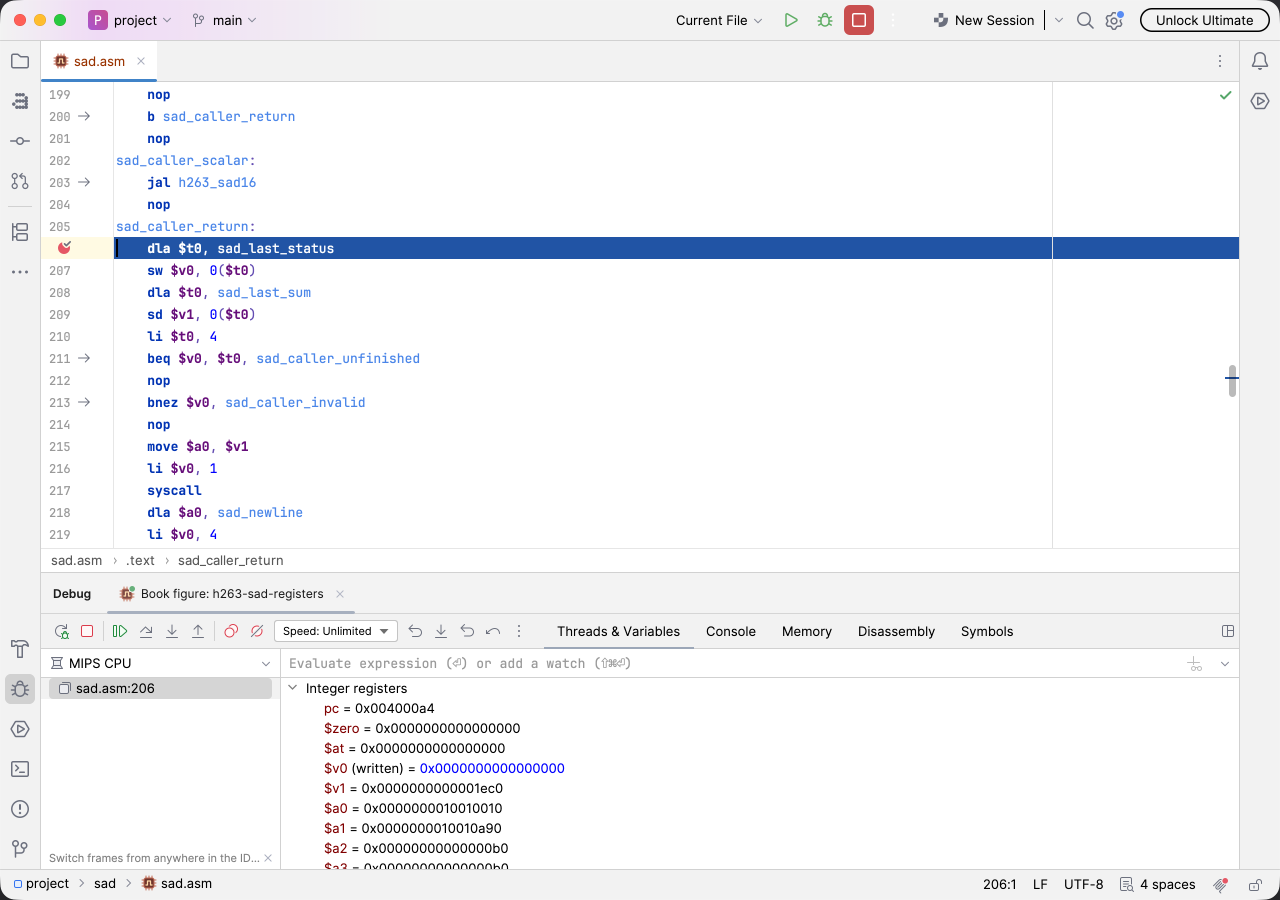
\includegraphics[artifact]{book/captures/035-h263/h263-sad-result/registers.png}}
\edef\MARSsadsourceLeft{\the\dimexpr0.036718750\wd0\relax}
\edef\MARSsadsourceBottom{\the\dimexpr0.707777778\ht0\relax}
\edef\MARSsadsourceRight{\the\dimexpr0.611718750\wd0\relax}
\edef\MARSsadsourceTop{\the\dimexpr0.236666667\ht0\relax}
\edef\MARSsadreturnsLeft{\the\dimexpr0.246093750\wd0\relax}
\edef\MARSsadreturnsBottom{\the\dimexpr0.110000000\ht0\relax}
\edef\MARSsadreturnsRight{\the\dimexpr0.553125000\wd0\relax}
\edef\MARSsadreturnsTop{\the\dimexpr0.838888889\ht0\relax}
\begin{tikzpicture}[alt={Two annotated IDE details at sad_caller_return, before dla t0 sad_last_status. Register v0 is zero and v1 is hexadecimal 1ec0, decimal 7872. The caller has not yet copied the returned values into its named memory fields.}]
\node[anchor=north west,inner sep=0,font=\small\bfseries] (source-title) at (6mm,0) {Return before the caller saves its results};
\node[anchor=north west,inner sep=0] (source) at ([yshift=-1mm]source-title.south west) {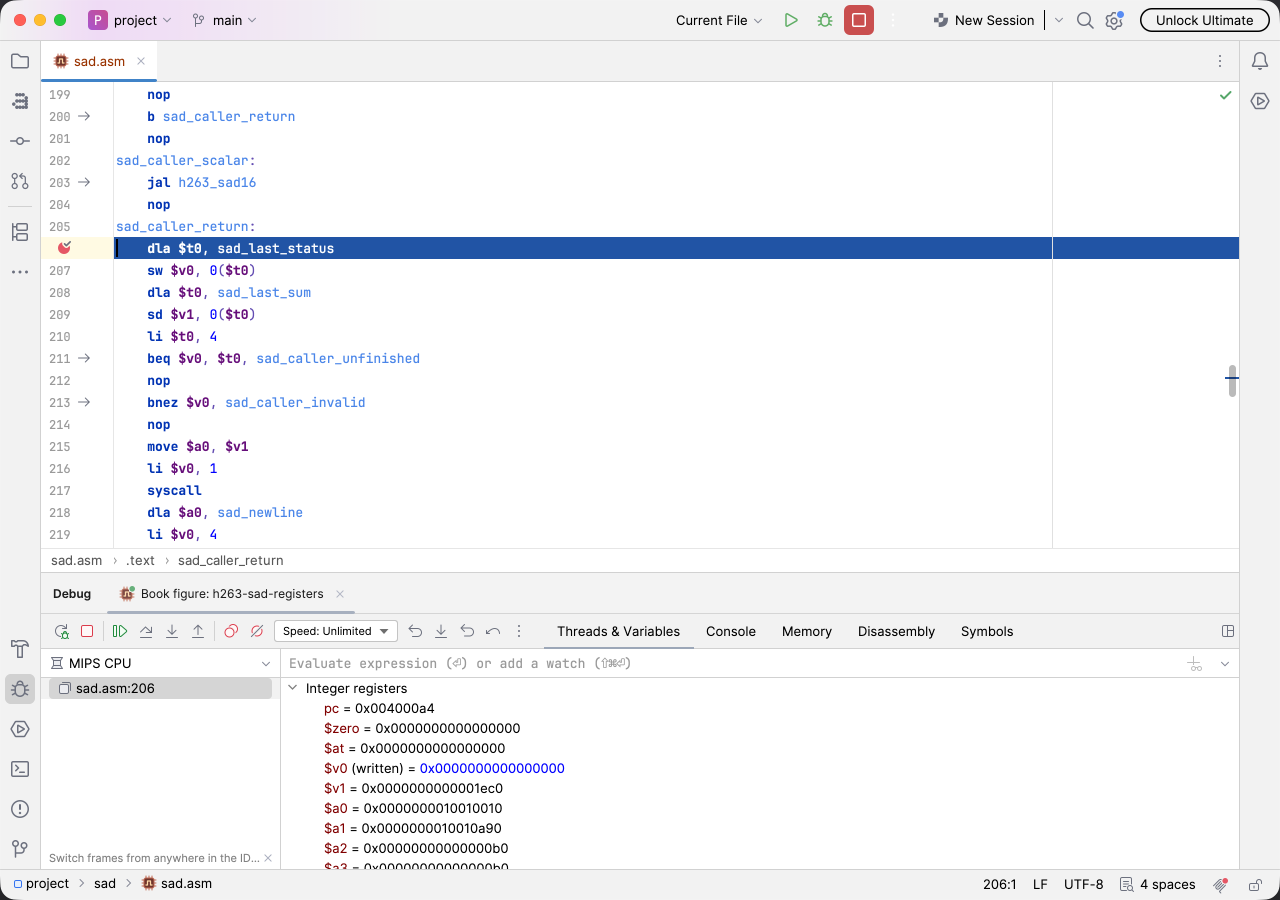
\includegraphics[width=0.7\linewidth,artifact,trim={\MARSsadsourceLeft{} \MARSsadsourceBottom{} \MARSsadsourceRight{} \MARSsadsourceTop{}},clip]{book/captures/035-h263/h263-sad-result/registers.png}};
\begin{scope}[shift={(source.south west)},x={($(source.south east)-(source.south west)$)},y={($(source.north west)-(source.south west)$)}]
\draw[black,line width=0.7pt] (0.153333333,0.080000000) rectangle (0.637777778,0.520000000);
\node[draw=black,fill=white,circle,inner sep=1.5pt,font=\footnotesize] at ($(0.153333333,0.520000000)+(-3mm,0)$) {1};
\end{scope}
\node[anchor=north west,inner sep=0,font=\small\bfseries] (returns-title) at ([yshift=-2mm]source.south west) {Success and an unsigned difference sum};
\node[anchor=north west,inner sep=0] (returns) at ([yshift=-1mm]returns-title.south west) {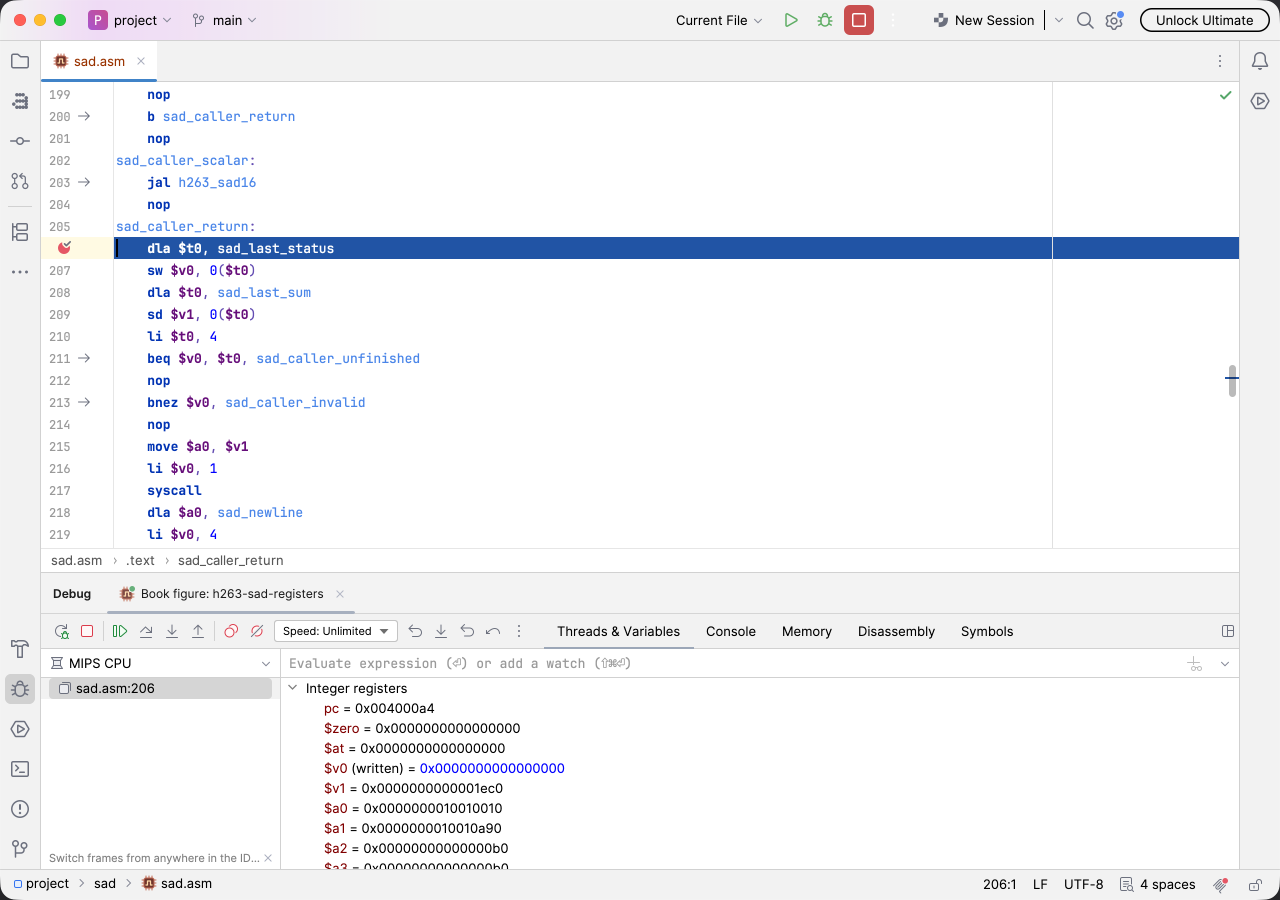
\includegraphics[width=0.5\linewidth,artifact,trim={\MARSsadreturnsLeft{} \MARSsadreturnsBottom{} \MARSsadreturnsRight{} \MARSsadreturnsTop{}},clip]{book/captures/035-h263/h263-sad-result/registers.png}};
\begin{scope}[shift={(returns.south west)},x={($(returns.south east)-(returns.south west)$)},y={($(returns.north west)-(returns.south west)$)}]
\draw[black,line width=0.7pt] (0.023346304,0.065217391) rectangle (0.976653696,0.934782609);
\node[draw=black,fill=white,circle,inner sep=1.5pt,font=\footnotesize] at ($(0.023346304,0.934782609)+(-3mm,0)$) {2};
\end{scope}
\end{tikzpicture}
\par\smallskip
\begin{minipage}{\linewidth}
\small
\begin{enumerate}
\item The highlighted \texttt{dla} is the next instruction. The SAD routine has returned, but the caller has not yet stored \texttt{sad\_last\_status} or \texttt{sad\_last\_sum}. Inspect the return registers at this boundary.
\item \texttt{\$v0}=0 reports success. \texttt{\$v1}=\texttt{0x1ec0}=7872 is the sum of absolute differences across all 256 active samples. It is neither a signed difference nor an average. The scalar and MSA modes must produce the same exact integer result.
\end{enumerate}
\end{minipage}
\caption{The completed MSA SAD kernel at its caller return. Two details come from one Debug screenshot.}
\label{fig:h263-sad-result}
\end{figure}
